\documentclass[14pt, fleqn, xcolor={dvipsnames, table}]{beamer}
\usepackage[T2A]{fontenc}
\usepackage[utf8]{inputenc}
\usepackage[english,russian]{babel}
\usepackage{amssymb,amsfonts,amsmath,mathtext}
\usepackage{cite,enumerate,float,indentfirst}
\usepackage{cancel}

\usepackage{tikz}                   
\usetikzlibrary{shadows}

% \usepackage{enumitem}
% \setitemize{label=\usebeamerfont*{itemize item}%
%   \usebeamercolor[fg]{itemize item}
%   \usebeamertemplate{itemize item}}

\graphicspath{{images/}}

\usetheme{Madrid}
\usecolortheme{seahorse}
\renewcommand{\CancelColor}{\color{red}}

\setbeamercolor{footline}{fg=Blue!50}
\setbeamertemplate{footline}{
  \leavevmode%
  \hbox{%
  \begin{beamercolorbox}[wd=.333333\paperwidth,ht=2.25ex,dp=1ex,center]{}%
    И. Кураленок, Н. Поваров, Яндекс
  \end{beamercolorbox}%
  \begin{beamercolorbox}[wd=.333333\paperwidth,ht=2.25ex,dp=1ex,center]{}%
    Санкт-Петербург, 2013
  \end{beamercolorbox}%
  \begin{beamercolorbox}[wd=.333333\paperwidth,ht=2.25ex,dp=1ex,right]{}%
  Стр. \insertframenumber{} из \inserttotalframenumber \hspace*{2ex}
  \end{beamercolorbox}}%
  \vskip0pt%
}
\newcommand\indentdisplays[1]{%
     \everydisplay{\addtolength\displayindent{#1}%
     \addtolength\displaywidth{-#1}}}
\newcommand{\itemi}{\item[\checkmark]}

\title{Линейные модели: уменьшаем variance\\\small{}}
\author[]{\small{%
И.~Куралёнок,
Н.~Поваров}}
\date{}

\begin{document}

\begin{frame}
\maketitle
\small
\begin{center}
\vspace{-60pt}
\normalsize {\color{red}Я}ндекс \\
\vspace{80pt}
\footnotesize СПб, 2013
\end{center}
\end{frame}

\section{Постановка задачи восстановления сигнала}
\subsection{Пример}
\subsection{Разложение сигнала в Фурье и постановка в нахождении коэффициентов}
\section{LASSO для восстановления сигнала}
\subsection{Теорема о качестве восстановленного сигнала (Candes et al. 2006)}
\subsection{Стабильность решения: RIP, RRfND (Candes et al. 2006)}
\subsection{LASSO persistency theorem (Bickel et al., 2009)}
\section{Support vector machines}
\subsection{Идея метода}
\begin{frame}{SVM(воспоминания о былом)}
\begin{itemize}
  \item Последний из линейных методов, который мы рассмотрим подробно.
  \item Rocket science до конца 90-х, по крайней мере в задачах классификации.
\end{itemize}
\end{frame}

\begin{frame}{SVM на пальцах}
\begin{itemize}
  \item Максимальный зазор.
  \item Нелинейные преобразования.
\end{itemize}
\begin{center}
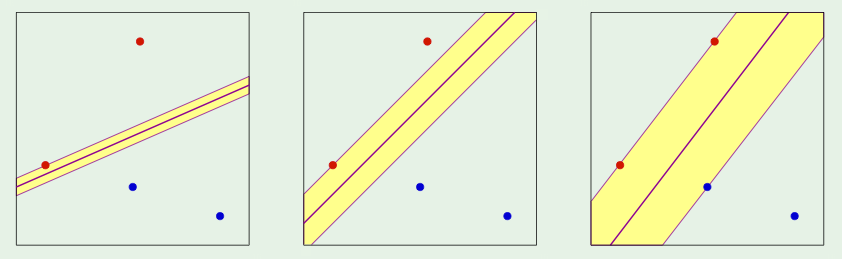
\includegraphics[width=0.9\textwidth]{SVM_1.png}
\end{center}
\end{frame}

\begin{frame}{Мысли вслух}
\begin{itemize}
  \item Почему большой зазор это хорошо?
  \item Какая $\beta$ максимизирует зазор? 
\end{itemize}
\end{frame}

\begin{frame}{Решение}
Ищем решение вида: \
$$
\beta^Tx - \beta_0 = 0,
$$ 
где $\beta$ - перпендикуляр к разделяющей плоскости. Для линейно-разделимых данных: \
$$
c_i(\beta x_i - \beta_0) \ge 1
$$
Ширина полосы: \
$$
\frac{2}{\|\beta\|}
$$
\end{frame}

\subsection{Коэффициенты Лагранжа для решения задачи про максимальное расстояние}
\begin{frame}{Лагранж}
По теореме Куна-Таккера: \
$$
\mathcal{L} = \frac{1}{2}\|\beta\|^2 - \sum_{i=1}^m\alpha_i(c_i(\beta x_i - \beta_0) - 1), \alpha_i \ge 0
$$ 
Сведём эту задачу к: \
$$
\left\{  
           \begin{array}{ll}  
            -\mathcal{L} = -\sum_{i=1}^m\alpha_i + \frac{1}{2}\sum_{i=1}^m\sum_{j=1}^m\alpha_i\alpha_jc_ic_j(x_ix_j) \\  
            \alpha_i \ge 0 & \\
            \sum_{i=1}^m\alpha_ic_i = 0
           \end{array}   
           \right.
$$
Тогда: \
$$\begin{array}{l}
\beta = \sum_{i=1}^m\alpha_ic_ix_i \\
\beta_0 = \beta x_i - c_i, \alpha_i > 0
\end{array}$$
\end{frame}

\subsection{Переход к дуальному решению}
\subsection{Идея как можно на халяву это решить}
\subsection{Kernel trick}
\subsection{Сведение SVM к регуляризации (основная идея)}
\end{document}
